\section{Details of the setup}
\label{app:setup-details}
\label{app:settings}

\paragraph{Outcomes.} Table~\ref{tab:outcomes} states the outcome rule of
Section~\ref{sec:setup}. Its boundaries suit the present setting, in which a
successful round takes a new length from zero to 70\% or more at once and an
unsuccessful one leaves it near zero; elsewhere they would have to be chosen
anew.

\begin{table}[htbp]
\centering
\caption{The outcome of a round at one problem length. Scores are accuracies
  on test problems, in percentage points. ``The best'' is the highest score
  any teacher's student reached at that length, in the same round and from the
  same starting model.}
\label{tab:outcomes}
\small
\begin{tabular}{@{}lll@{}}
\toprule
Length & Outcome & Condition \\
\midrule
Could already do & Did nothing & Changes by at most 3 points \\
 & Did harm & Falls by more than 3 points, here or on easy problems \\
\addlinespace
New & Paid off & Rises by at least 20 points, to within 10 of the best \\
 & Taught wrong answers & Rises, but ends 30 points or more below the best \\
 & \quad (counted as harm) & \\
 & Did little or nothing & Rises by less than 10 points \\
\bottomrule
\end{tabular}
\end{table}


\paragraph{Adjustments before the freeze.}
Four adjustments were made between the calibration runs and the freeze.
First, we placed novelty ahead of agreement, which raised the number of
correctly predicted calibration cases from 107 to 166 of 176. Second, we
increased the number of splits for 13- to 15-digit problems from three to
five, because three splits artificially depressed the confirmed share of an
otherwise sound teacher. Third, we added the 10-point and 50\% conditions to
the outcome rule. Fourth, we added the requirement that at least 5\% of
answers be kept, which guards against sampling noise: when a teacher keeps
fewer than a hundred answers, the proportion of new ones varies widely
between samples.


\paragraph{Reproduction.}
Table~\ref{tab:reproduction} compares our accuracies with those reported by
\citet{shin2026compositional}. The two are not directly comparable: they
train for eight rounds and test up to 23 digits, whereas we train for four
and test up to 15. Within those limits the pattern is the same. With their
filter the model reaches nearly full accuracy at every length it has been
taught, and without it accuracy remains far lower.

% Generated by `uv run python -m gainpred.writeup`; do not edit by hand.
\begin{table}[H]
\centering
\caption{Accuracy (\%) on the reproduction test set: 100 problems per length, 3
  to 15 digits, greedy answers, scored after all experiments on the saved models
  of the evaluation runs (mean of three runs, range in brackets). Shin et al.'s
  figures are those they report (their Table 10 and appendix C.1); they train 8
  rounds up to 23 digits and test up to 23 digits, so their columns cover 8-23
  and 23 digits, ours 8-15 and 15 digits. The no-carry rule corresponds to their
  filtered composition, no selection to their unfiltered composition.}
\label{tab:reproduction}
\small
\begin{tabular}{lrr}
\toprule
Model & Mean over new lengths & Longest length \\
\midrule
This paper (8--15 digits; 15 digits) &  &  \\
Starting model & 1.8 (0.4--3.5) & 0.0 (0.0--0.0) \\
No-carry rule, round 1 & 31.5 (27.0--37.1) & 0.0 (0.0--0.0) \\
No-carry rule, round 2 & 59.5 (56.8--61.3) & 0.0 (0.0--0.0) \\
No-carry rule, round 3 & 84.5 (84.2--85.0) & 0.0 (0.0--0.0) \\
No-carry rule, round 4 & 99.6 (98.9--100.0) & 99.0 (98.0--100.0) \\
No selection, round 1 & 10.8 (10.5--11.0) & 0.0 (0.0--0.0) \\
No selection, round 2 & 25.2 (24.8--26.2) & 0.0 (0.0--0.0) \\
No selection, round 3 & 40.8 (39.0--41.9) & 0.0 (0.0--0.0) \\
No selection, round 4 & 41.8 (36.0--44.9) & 24.0 (17.0--28.0) \\
\midrule
Shin et al. (8--23 digits; 23 digits) &  &  \\
Starting model & 0.0 & 0.0 \\
Filtered composition, last round (8) & 93.7 & 80.0 \\
Unfiltered composition, last round (8) & 33.5 & 11.0 \\
\bottomrule
\end{tabular}
\end{table}



\section{Further results on the predictions}
\label{app:prediction}

This section contains the material referred to in
Section~\ref{sec:do-the-checks-predict} of the paper: the kinds of case
(Table~\ref{tab:p9b-cases}), the margins of the checks
(Figure~\ref{fig:checks}), the cases from weak starting models
(Table~\ref{tab:weak}), the cases without an outcome
(Table~\ref{tab:no-outcome}), the comparison with training briefly
(Tables~\ref{tab:baseline} and~\ref{tab:cost-addition}), and the agreement
rule against the no-carry rule
(Figure~\ref{fig:exp1}).

% Generated by `uv run python -m gainpred.writeup`; do not edit by hand.
\begin{table}[t]
\centering
\caption{Cases correctly predicted, by kind of case, in the evaluation runs.}
\label{tab:p9b-cases}
\small
\begin{tabular}{lrr}
\toprule
Kind of case & Cases & Correctly predicted \\
\midrule
Agreement rule, new lengths & 14 & 14 \\
No-carry rule, new lengths & 14 & 14 \\
No selection & 60 & 60 \\
Sample and vote & 60 & 60 \\
Lengths already learned & 79 & 79 \\
Starting model stopped early (weak) & 10 & 1 \\
New length started midway & 3 & 3 \\
No selection after the no-carry rule (run f) & 18 & 18 \\
\bottomrule
\end{tabular}
\end{table}


\paragraph{Margins.}
Figure~\ref{fig:checks} shows why these predictions are robust. The values of
each check form two clusters, and the threshold lies in the gap between them.
Leaving aside the cases decided by the 5\% minimum, novelty was at most
\gpNoveltyMarginLow\% wherever the prediction was ``does nothing'' and at
least \gpNoveltyMarginHigh\% everywhere else. The confirmed share was at most
\gpConfirmedMarginLow\% in the \gpConfirmedHarmCases{} cases it predicted to
do harm, and at least \gpConfirmedMarginHigh\% in the \gpConfirmedPaysCases{}
it predicted to pay off. Any thresholds within these ranges yield the same
predictions. We computed the ranges after the evaluation runs; the
thresholds themselves were fixed beforehand.

% Generated by `uv run python -m gainpred.writeup`; do not edit by hand.
\begin{figure}[htbp]
\centering
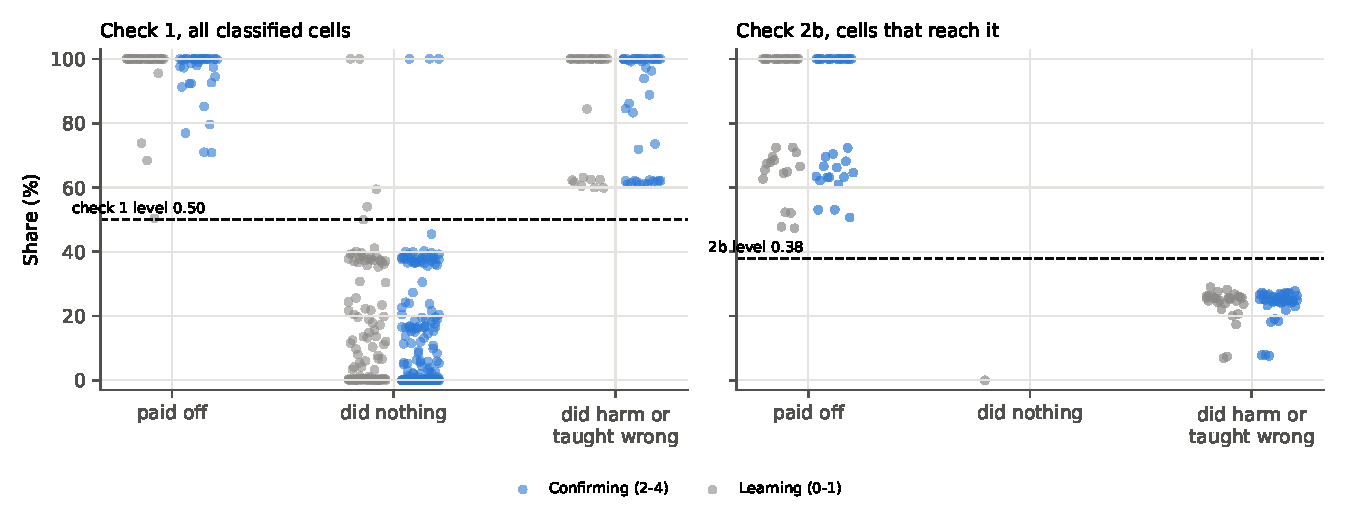
\includegraphics[width=\linewidth]{generated/figure_checks.pdf}
\caption{Novelty (all cases with an outcome) and confirmed share (cases that
  reach the agreement check) by outcome. Dashed: the levels fixed before the
  evaluation runs. Shaded: the range within which a level gives the same
  predictions on the evaluation runs (computed after them).}
\label{fig:checks}
\end{figure}


\paragraph{The basics check.} Ten cases with an outcome come from starting
models that fail the basics check, so the rule predicted harm in all ten. It
was right once (Table~\ref{tab:weak}). Three of
these models were just below the pass mark, with at least 91\% on every size
of easy problem. All six of their cases paid off, as they do for a fully
trained starting model. The other three failed some sizes of easy problem
almost entirely. Their rounds mostly did little, and taught wrong answers in
one case. Weak basics therefore did not predict harm in our runs.

The measurements of Section~\ref{sec:confirmed-right} explain why. A model
just below the pass mark still yields a teacher that is mostly right, and its
rounds pay off. A much weaker model yields a teacher whose accuracy varies
sharply from one length to the next, from \gpTaWeakAccLow\% to
\gpTaWeakAccHigh\%, and its confirmed share fell with that accuracy, to
\gpTaWeakConfirmedLow\%. What the basics check was intended to establish, the
agreement check establishes more directly, on the hard problems themselves.
Without the basics check, the two other checks would have been correct in
\gpCorrectNoBasics{} of \gpCases{} cases (\gpCorrectNoBasicsPct\%). We
computed this after the evaluation runs, and the rule as frozen remains our
main result.

One of the remaining errors is a failure of imitation
(Section~\ref{sec:what-changes}). At 8 digits, one of the very weak models
yielded a teacher that was right on nearly all of its kept answers, and the
student's accuracy nevertheless rose by less than 10 points. A teacher can be
right and the student unable to follow.

% Generated by `uv run python -m gainpred.writeup`; do not edit by hand.
\begin{table}[htbp]
\centering
\caption{The 12 cases from weak starting models (stopped early), evaluation
  runs, including those without an outcome. Easy: lowest accuracy (\%) over easy
  sizes 3-7 before the round (the basics check needs 98\% at every size).
  Before, after: accuracy (\%) at that length; best: the best teacher's after,
  same starting model and round.}
\label{tab:weak}
\small
\resizebox{\linewidth}{!}{%
\begin{tabular}{lrrrrrlll}
\toprule
Starting model & Easy & Length & Before & After & Best & Outcome & Prediction
  & Without basics \\
\midrule
2 (1,425 updates) & 4.7 & 8 & 0.2 & 85.5 & 100.0 & without an outcome
  & does harm & pays off \\
2 (1,425 updates) & 4.7 & 9 & 0.0 & 39.0 & 100.0 & taught wrong answers
  & does harm & does harm \\
2 (2,200 updates) & 91.8 & 8 & 14.9 & 98.3 & 100.0 & paid off & does harm
  & pays off \\
2 (2,200 updates) & 91.8 & 9 & 0.0 & 96.2 & 100.0 & paid off & does harm
  & pays off \\
3 (3,450 updates) & 97.8 & 8 & 0.0 & 98.0 & 99.8 & paid off & does harm
  & pays off \\
3 (3,450 updates) & 97.8 & 9 & 0.0 & 95.3 & 100.0 & paid off & does harm
  & pays off \\
3 (3,500 updates) & 0.3 & 8 & 0.0 & 8.5 & 99.8 & did nothing & does harm
  & pays off \\
3 (3,500 updates) & 0.3 & 9 & 0.0 & 0.6 & 100.0 & did nothing & does harm
  & does harm \\
4 (2,250 updates) & 96.1 & 8 & 24.1 & 97.0 & 99.2 & paid off & does harm
  & pays off \\
4 (2,250 updates) & 96.1 & 9 & 0.0 & 92.8 & 98.3 & paid off & does harm
  & pays off \\
4 (3,000 updates) & 0.9 & 8 & 0.2 & 78.4 & 99.2 & without an outcome & does harm
  & pays off \\
4 (3,000 updates) & 0.9 & 9 & 0.0 & 7.4 & 98.3 & did nothing & does harm
  & does harm \\
\bottomrule
\end{tabular}
}
\end{table}

% Generated by `uv run python -m gainpred.writeup`; do not edit by hand.
\begin{table}[H]
\centering
\caption{The 12 evaluation cases without an outcome, and the gap in the outcome
  rule each falls in. Before, after: accuracy (\%) at that length; novelty in
  \%.}
\label{tab:no-outcome}
\small
\resizebox{\linewidth}{!}{%
\begin{tabular}{llrrrrrll}
\toprule
Teacher & Starting model & Round & Length & Before & After & Novelty
  & Prediction & Gap in the outcome rule \\
\midrule
Agreement rule & 2 & 2 & 10 & 78.6 & 99.8 & 27.5 & does nothing
  & started above 50\%, rose more than 3 points \\
Agreement rule & 3 & 2 & 10 & 79.2 & 99.8 & 18.1 & does nothing
  & started above 50\%, rose more than 3 points \\
Agreement rule & 3 & 3 & 12 & 96.2 & 100.0 & 3.9 & does nothing
  & started above 50\%, rose more than 3 points \\
Agreement rule & 4 & 2 & 10 & 91.1 & 98.5 & 5.4 & does nothing
  & started above 50\%, rose more than 3 points \\
No-carry rule & 2 (weak) & 1 & 8 & 0.2 & 85.5 & 100.0 & does harm
  & rose 20 points or more, 10-30 below the best \\
No-carry rule & 2 & 3 & 12 & 62.6 & 100.0 & 30.6 & does nothing
  & started above 50\%, rose more than 3 points \\
No-carry rule & 2 & 4 & 14 & 93.0 & 100.0 & 6.6 & does nothing
  & started above 50\%, rose more than 3 points \\
No-carry rule & 3 & 3 & 12 & 79.2 & 100.0 & 23.6 & does nothing
  & started above 50\%, rose more than 3 points \\
No-carry rule & 3 & 4 & 14 & 90.6 & 100.0 & 10.0 & does nothing
  & started above 50\%, rose more than 3 points \\
No-carry rule & 4 (weak) & 1 & 8 & 0.2 & 78.4 & 99.9 & does harm
  & rose 20 points or more, 10-30 below the best \\
No-carry rule & 4 & 2 & 10 & 58.3 & 98.4 & 41.9 & does nothing
  & started above 50\%, rose more than 3 points \\
No-carry rule & 4 & 4 & 14 & 93.5 & 98.8 & 6.3 & does nothing
  & started above 50\%, rose more than 3 points \\
\bottomrule
\end{tabular}
}
\end{table}


\paragraph{Compared with training briefly.}
\label{sec:vs-baseline}
\label{sec:baselines}
We compare the prediction rule with two baselines. The first always predicts
the most frequent outcome. The second is the obvious alternative to checks:
start the round, train for 200 of the 3,000 updates, measure accuracy on the
test set, and extrapolate from the early change. We defined this baseline
after the evaluation runs; its thresholds were tuned on the calibration runs
and recorded before any of its results on the evaluation runs were read.
Unlike our checks, it requires correct answers to the hard problems.

Computational cost is measured as wall-clock time on a single GPU. For each
round, we compare the time needed to run the checks with the total time of
the round, that is, generating the kept answers and training on them.

The obvious alternative is to start the round and inspect it
. As originally run, this baseline was correct
in \gpBaselineCorrect{} of \gpCases{} cases (\gpBaselineCorrectPct\%). A
variant that we defined after the evaluation runs, in the baseline's favor,
reached \gpVariantCorrect{} (\gpVariantCorrectPct\%), still below the checks
(Table~\ref{tab:baseline}). The baseline missed harmful cases: it flagged
\gpBaselineHarmFlagged{} of \gpHarmful{}, and the variant
\gpVariantHarmFlagged{}, whereas the checks flagged all \gpHarmful{}. It
outperformed the checks on the \gpWeakCases{} cases from weak starting
models, with \gpBaselineWeakCorrect{} and \gpVariantWeakCorrect{} correct
against \gpOursWeakCorrect{}, because it does not rely on the basics check.

% Generated by `uv run python -m gainpred.writeup`; do not edit by hand.
\begin{table}[t]
\centering
\caption{Cells matched by our checks (before training, no reference answers) and by the baseline (200 updates, then accuracy on the test problems, which needs their reference answers), confirming runs. Baseline levels fitted on starting points 0-1: G = 15, H = 47, D = 51. Cost per round: checks 9\%, baseline 56\% of a full round.}
\label{tab:baseline}
\small
\begin{tabular}{lrrr}
\toprule
 & Cells & Our checks & Baseline \\
\midrule
All cells & 258 & 249 & 224 \\
Paid off & 37 & 31 & 32 \\
Did nothing & 178 & 175 & 154 \\
Did harm or taught wrong answers & 43 & 43 & 38 \\
Agreement rule, new lengths & 14 & 14 & 14 \\
No-carry rule, new lengths & 14 & 14 & 12 \\
No selection & 60 & 60 & 55 \\
Sample and vote & 60 & 60 & 39 \\
Lengths already learned & 79 & 79 & 79 \\
Starting model stopped early (weak) & 10 & 1 & 4 \\
New length started midway & 3 & 3 & 3 \\
No selection after the no-carry rule (run f) & 18 & 18 & 18 \\
\bottomrule
\end{tabular}
\end{table}


The baseline is also more expensive and more demanding. It took
\gpBaselineCostAdditionPct\% of the computing time of a round, because it must first
build the round's training answers, and it requires correct answers to the
hard problems. The checks took \gpChecksCostAdditionPct\%
(Table~\ref{tab:cost-addition}) and require none. Rounds are short in this
setting, so these proportions would differ with longer training: the cost of
the checks depends on the number of problems examined, not on the length of
training.

% Generated by `uv run python -m gainpred.writeup`; do not edit by hand.
\begin{table}[htbp]
\centering
\caption{Seconds per round on one A10 GPU, evaluation runs on addition: whole
  round (build, replay, checks, 3,000 updates; evaluation not timed) and the
  checks alone.}
\label{tab:cost-addition}
\small
\begin{tabular}{lrrrr}
\toprule
Teacher & Rounds & Round s & Checks s & Checks \% \\
\midrule
No-carry rule & 12 & 309 & 34 & 11 \\
Agreement rule & 12 & 573 & 49 & 9 \\
No selection & 12 & 282 & 34 & 12 \\
Sample and vote & 12 & 932 & 52 & 6 \\
No selection after the no-carry rule & 3 & 310 & 40 & 13 \\
No-carry rule, weak starting models & 6 & 195 & 10 & 5 \\
\bottomrule
\end{tabular}
\end{table}


\paragraph{Agreement against the hand-written filter.}
\label{sec:agreement-vs-filter}

The agreement rule keeps an answer whenever two splits produce it, and
encodes no knowledge of carrying. After four rounds, the resulting student
was on average within \gpGapMean{} percentage points of the student trained
with the no-carry rule at every length from 8 to 15 digits
(Figure~\ref{fig:exp1}; Table~\ref{tab:passmark}), and trailed it by at most \gpGapWorst{} points in
the worst single run. Even on problems with a carry across the first split,
the largest gaps were \gpGapMeanCarry{} points on average and
\gpGapWorstCarry{} points in the worst run. We had not specified in advance
how closely the two had to match.

% Generated by `uv run python -m gainpred.writeup`; do not edit by hand.
\begin{figure}[htbp]
\centering
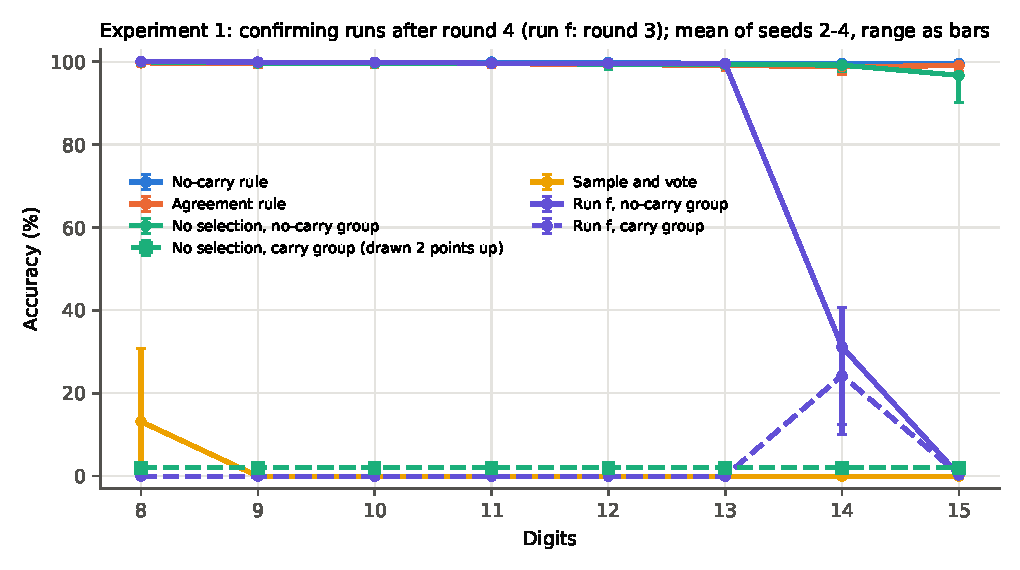
\includegraphics[width=\linewidth]{generated/figure_exp1.pdf}
\caption{Accuracy after round 4 (no selection after the no-carry rule: after its
  one round, round 3), evaluation runs; mean over the three starting models,
  range as bars.}
\label{fig:exp1}
\end{figure}


The measurements of Section~\ref{sec:confirmed-right} explain how this is
possible. Agreement does not require a teacher that is usually right. With no
selection, the first split's answer was correct in only
\gpTaNoSelectAccLow--\gpTaNoSelectAccHigh\% of cases, yet the answers that
another split confirmed were correct in at least
\gpTaNoSelectAccConfirmedLow\%. The agreement rule keeps such answers and
discards the rest, and its kept answers were correct in at least
\gpTaAgreementAccLow\% of cases. A filter written for the task encodes why an
answer is wrong. Agreement relies only on wrong answers not recurring from
one split to the next, which on this task was sufficient.

Dispensing with a hand-written filter has a cost. Because the agreement rule
must construct each answer several times, it took \gpBuildRatio{} times as
long as the no-carry rule to fill the same training quota. It also yields a
skewed sample: whereas roughly \gpNaturalCarryLow\% of fresh problems have a
carry at the first split, only \gpKeptAgreementLow\% to
\gpKeptAgreementHigh\% of the answers kept by the agreement rule do. Splits
are most likely
to agree when none of them errs, which removes the hardest cases
disproportionately. Finally, the rule presupposes a second valid way of
splitting the problem.

\citet{shin2026compositional} leave open how a composition procedure can be
validated without a task-specific filter. For addition, agreement across
splits provides one practical answer.

% Generated by `uv run python -m gainpred.writeup`; do not edit by hand.
\begin{table}[htbp]
\centering
\caption{Agreement rule minus no-carry rule after round 4, points, evaluation
  runs: mean over three starting models and worst single run (its starting
  model).}
\label{tab:passmark}
\small
\begin{tabular}{lrrrr}
\toprule
Digits & Mean gap & Worst run & Mean gap, carry & Worst run, carry \\
\midrule
8 & -0.2 & -0.5 (4) & -0.4 & -0.9 (4) \\
9 & -0.3 & -0.7 (4) & -0.4 & -1.1 (4) \\
10 & -0.3 & -0.8 (4) & -0.5 & -1.4 (4) \\
11 & -0.4 & -1.1 (4) & -0.5 & -1.3 (4) \\
12 & -0.5 & -1.3 (4) & -0.8 & -2.2 (4) \\
13 & -0.5 & -1.0 (4) & -1.0 & -1.8 (4) \\
14 & -0.8 & -1.8 (4) & -1.3 & -3.1 (4) \\
15 & -0.5 & -1.2 (4) & -1.1 & -2.2 (4) \\
\bottomrule
\end{tabular}
\end{table}


\section{The ladder: further details}
\label{app:ladder-more}

This section supplements Section~\ref{sec:ladder} of the paper.
Table~\ref{tab:ladder-splits} lists the three splits of every length.
Table~\ref{tab:ladder-lengths} gives, for every length and seed, the final
accuracy of the arm that builds answers everywhere and of the self-paced
arm, with the novelty the self-paced arm measured and what it then did.

% Generated by `uv run python -m gainpred.ladder_paper`; do not edit by hand.
\begin{table}[htbp]
\centering
\caption{The three splits of every length 8--39, each written as left piece +
  right piece (digits).}
\label{tab:ladder-splits}
\small
\setlength{\tabcolsep}{3pt}
\begin{tabular}{rlll@{\hspace{1.5em}}rlll}
\toprule
\multicolumn{4}{c}{8--23 digits} & \multicolumn{4}{c}{24--39 digits} \\
\cmidrule(lr){1-4}\cmidrule(lr){5-8}
Digits & Split 1 & Split 2 & Split 3 & Digits & Split 1 & Split 2 & Split 3 \\
\midrule
8 & 3 + 5 & 4 + 4 & 5 + 3 & 24 & 11 + 13 & 12 + 12 & 13 + 11 \\
9 & 3 + 6 & 4 + 5 & 5 + 4 & 25 & 11 + 14 & 12 + 13 & 13 + 12 \\
10 & 4 + 6 & 5 + 5 & 6 + 4 & 26 & 12 + 14 & 13 + 13 & 14 + 12 \\
11 & 4 + 7 & 5 + 6 & 6 + 5 & 27 & 12 + 15 & 13 + 14 & 14 + 13 \\
12 & 5 + 7 & 6 + 6 & 7 + 5 & 28 & 13 + 15 & 14 + 14 & 15 + 13 \\
13 & 5 + 8 & 6 + 7 & 7 + 6 & 29 & 13 + 16 & 14 + 15 & 15 + 14 \\
14 & 6 + 8 & 7 + 7 & 8 + 6 & 30 & 14 + 16 & 15 + 15 & 16 + 14 \\
15 & 6 + 9 & 7 + 8 & 8 + 7 & 31 & 14 + 17 & 15 + 16 & 16 + 15 \\
\midrule
16 & 7 + 9 & 8 + 8 & 9 + 7 & 32 & 15 + 17 & 16 + 16 & 17 + 15 \\
17 & 7 + 10 & 8 + 9 & 9 + 8 & 33 & 15 + 18 & 16 + 17 & 17 + 16 \\
18 & 8 + 10 & 9 + 9 & 10 + 8 & 34 & 16 + 18 & 17 + 17 & 18 + 16 \\
19 & 8 + 11 & 9 + 10 & 10 + 9 & 35 & 16 + 19 & 17 + 18 & 18 + 17 \\
20 & 9 + 11 & 10 + 10 & 11 + 9 & 36 & 17 + 19 & 18 + 18 & 19 + 17 \\
21 & 9 + 12 & 10 + 11 & 11 + 10 & 37 & 17 + 20 & 18 + 19 & 19 + 18 \\
22 & 10 + 12 & 11 + 11 & 12 + 10 & 38 & 18 + 20 & 19 + 19 & 20 + 18 \\
23 & 10 + 13 & 11 + 12 & 12 + 11 & 39 & 18 + 21 & 19 + 20 & 20 + 19 \\
\bottomrule
\end{tabular}
\end{table}

% Generated by `uv run python -m gainpred.ladder_paper`; do not edit by hand.
\begin{table}[htbp]
\centering
\caption{For each length and seed: final accuracy (\%) of the third arm (Agreed)
  and of the self-paced arm (Paced) after their last round, the self-paced arm's
  novelty in its check before the length's round (\% of pair-agreed answers that
  differ from the direct answer), and whether it built or skipped the length.}
\label{tab:ladder-lengths}
\scriptsize
\setlength{\tabcolsep}{3pt}
\begin{tabular}{rrrrlrrrlrrrl}
\toprule
 & \multicolumn{4}{c}{Seed 5} & \multicolumn{4}{c}{Seed 6}
 & \multicolumn{4}{c}{Seed 7} \\
\cmidrule(lr){2-5}\cmidrule(lr){6-9}\cmidrule(lr){10-13}
Digits & Agreed & Paced & Novelty & Paced did & Agreed & Paced & Novelty
  & Paced did & Agreed & Paced & Novelty & Paced did \\
\midrule
8 & 98.8 & 99.7 & 96.5 & built & 100.0 & 100.0 & 82.5 & built & 100.0 & 100.0
  & 100.0 & built \\
9 & 99.0 & 99.6 & 100.0 & built & 100.0 & 100.0 & 100.0 & built & 99.9 & 100.0
  & 100.0 & built \\
10 & 98.8 & 99.4 & 85.8 & built & 100.0 & 100.0 & 72.5 & built & 100.0 & 100.0
  & 100.0 & built \\
11 & 98.8 & 99.6 & 100.0 & built & 100.0 & 99.9 & 100.0 & built & 100.0 & 100.0
  & 100.0 & built \\
12 & 99.0 & 99.6 & 92.8 & built & 100.0 & 100.0 & 0.57 & skipped & 100.0 & 100.0
  & 40.6 & built \\
13 & 98.6 & 99.2 & 100.0 & built & 100.0 & 100.0 & 99.0 & built & 100.0 & 100.0
  & 100.0 & built \\
14 & 98.2 & 99.3 & 15.3 & built & 100.0 & 99.9 & 1.3 & skipped & 100.0 & 100.0
  & 0.15 & skipped \\
15 & 98.3 & 99.3 & 97.7 & built & 100.0 & 100.0 & 92.8 & built & 100.0 & 100.0
  & 100.0 & built \\
\midrule
16 & 97.8 & 99.2 & 12.4 & built & 100.0 & 100.0 & 0.00 & skipped & 100.0 & 100.0
  & 23.5 & built \\
17 & 98.1 & 99.4 & 89.1 & built & 100.0 & 100.0 & 28.5 & built & 100.0 & 100.0
  & 100.0 & built \\
18 & 97.6 & 98.6 & 2.9 & built & 100.0 & 100.0 & 0.15 & skipped & 100.0 & 100.0
  & 0.00 & skipped \\
19 & 97.1 & 98.4 & 99.4 & built & 100.0 & 100.0 & 0.15 & skipped & 100.0 & 100.0
  & 12.2 & built \\
20 & 98.2 & 99.5 & 0.29 & skipped & 100.0 & 100.0 & 51.8 & built & 100.0 & 100.0
  & 0.00 & skipped \\
21 & 97.6 & 99.0 & 4.9 & built & 100.0 & 100.0 & 100.0 & built & 99.9 & 100.0
  & 69.5 & built \\
22 & 97.4 & 98.5 & 0.30 & skipped & 100.0 & 99.9 & 0.00 & skipped & 99.9 & 100.0
  & 0.00 & skipped \\
23 & 97.8 & 98.8 & 12.7 & built & 100.0 & 100.0 & 1.4 & skipped & 100.0 & 100.0
  & 73.6 & built \\
\midrule
24 & 97.5 & 99.0 & 0.00 & skipped & 100.0 & 100.0 & 71.1 & built & 100.0 & 100.0
  & 0.15 & skipped \\
25 & 96.7 & 98.4 & 0.75 & skipped & 100.0 & 100.0 & 100.0 & built & 99.9 & 100.0
  & 79.3 & built \\
26 & 97.0 & 98.6 & 77.8 & built & 99.9 & 100.0 & 0.00 & skipped & 99.9 & 100.0
  & 0.14 & skipped \\
27 & 96.2 & 98.0 & 100.0 & built & 100.0 & 100.0 & 0.14 & skipped & 100.0
  & 100.0 & 24.4 & built \\
28 & 96.2 & 98.4 & 0.60 & skipped & 99.9 & 99.9 & 9.6 & built & 100.0 & 99.8
  & 0.00 & skipped \\
29 & 96.4 & 97.9 & 12.1 & built & 100.0 & 100.0 & 94.3 & built & 100.0 & 100.0
  & 32.7 & built \\
30 & 96.6 & 98.0 & 0.44 & skipped & 100.0 & 100.0 & 0.14 & skipped & 99.8
  & 100.0 & 0.00 & skipped \\
31 & 96.0 & 98.0 & 2.5 & built & 100.0 & 100.0 & 0.43 & skipped & 100.0 & 100.0
  & 1.3 & skipped \\
\midrule
32 & 95.0 & 97.9 & 0.30 & skipped & 100.0 & 100.0 & 2.3 & built & 99.9 & 100.0
  & 42.2 & built \\
33 & 95.7 & 97.8 & 1.3 & skipped & 100.0 & 100.0 & 66.1 & built & 99.9 & 100.0
  & 99.4 & built \\
34 & 96.0 & 98.0 & 1.2 & skipped & 100.0 & 100.0 & 0.59 & skipped & 100.0
  & 100.0 & 0.00 & skipped \\
35 & 95.2 & 97.6 & 75.1 & built & 99.9 & 100.0 & 7.1 & built & 100.0 & 100.0
  & 0.71 & skipped \\
36 & 95.0 & 97.3 & 1.2 & skipped & 99.9 & 100.0 & 0.00 & skipped & 99.9 & 99.9
  & 11.4 & built \\
37 & 95.5 & 97.7 & 1.7 & skipped & 99.9 & 100.0 & 2.4 & built & 100.0 & 100.0
  & 100.0 & built \\
38 & 95.2 & 97.5 & 21.7 & built & 99.9 & 100.0 & 0.00 & skipped & 100.0 & 99.8
  & 0.00 & skipped \\
39 & 95.2 & 97.8 & 89.0 & built & 100.0 & 100.0 & 0.14 & skipped & 100.0 & 99.4
  & 0.30 & skipped \\
\bottomrule
\end{tabular}
\end{table}


\paragraph{Training within a round.} Figure~\ref{fig:ladder-loss} shows the
training loss and the gradient norm during round~8, the round that adds 22
and 23 digits, for the run that diverged, its repetition, the self-paced arm
on the same seed, and the third arm on the two other seeds. In every run the
loss moves between about 0.01 and 1 and the gradient norm stays far above
the clipping level for the first two thirds of the round, while the learning
rate is constant; the loss falls only once the learning rate decays. The run
that diverged took one more such jump as the decay began and did not
recover.

\begin{figure}[htbp]
\centering
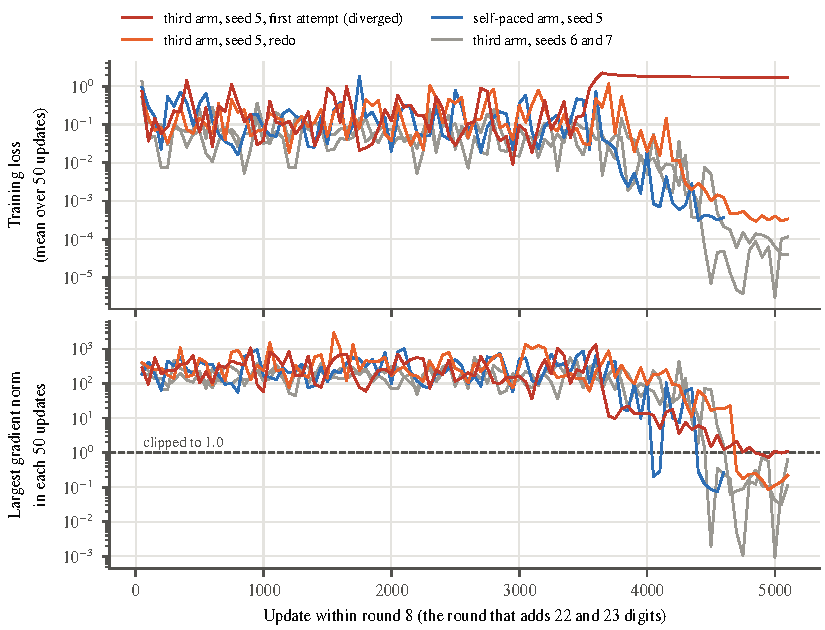
\includegraphics[width=\linewidth]{generated/figure_ladder_loss.pdf}
\caption{Training loss (top) and largest gradient norm before clipping
  (bottom) during round~8 of the ladder, per 50 updates.}
\label{fig:ladder-loss}
\end{figure}

